\documentclass{article}
\usepackage{fancyhdr}
\usepackage{ctex}
\usepackage{listings}
\usepackage{graphicx}
\usepackage[a4paper, body={18cm,22cm}]{geometry}
\usepackage{amsmath,amssymb,amstext,wasysym,enumerate,graphicx}
\usepackage{float,abstract,booktabs,indentfirst,amsmath}
\usepackage{array}
\usepackage{booktabs}
\usepackage{multirow}
\usepackage{url}
\usepackage{diagbox}
\renewcommand\arraystretch{1.4}
\usepackage{indentfirst}
\setlength{\parindent}{2em}
\usepackage{enumitem}
\setmonofont{Consolas}
\usepackage{listings}
\usepackage{xcolor}
\usepackage{makecell}
\setCJKmonofont{黑体}
\usepackage{tikz}
\usetikzlibrary{positioning, arrows.meta}
\lstset{
    % language = C,
    xleftmargin = 3em,xrightmargin = 3em, aboveskip = 1em,
	backgroundcolor = \color{white}, % 背景色
	basicstyle = \small\ttfamily, % 基本样式 + 小号字体
	rulesepcolor= \color{gray}, % 代码块边框颜色
	breaklines = true, % 代码过长则换行
	numbers = left, % 行号在左侧显示
	numberstyle = \small, % 行号字体
    numbersep = -14pt, 
    keywordstyle=\color{purple}\bfseries, % 关键字颜色
    commentstyle =\color{red!50!green!50!blue!60}, % 注释颜色
    stringstyle = \color{red}, % 字符串颜色
    morekeywords={ASSERT, int64_t, uint32_t},
	frame = shadowbox, % 用(带影子效果)方框框住代码块
	showspaces = false, % 不显示空格
	columns = fixed, % 字间距固定
} 
\lstset{
    sensitive=true,
    moreemph={ASSERT, NULL}, emphstyle=\color{red}\bfseries,
    moreemph=[2]{int64_t, uint32_t, tid_t, uint8_t, int16_t, uint16_t, int32_t, size_t}, emphstyle=[2]\color{purple}\bfseries,
    }
%--------------------页眉--------------------%
\pagestyle{fancy}
\fancyhead[L]{}
\fancyhead[R]{}
\fancyhead[C]{华东师范大学软件工程学院实验报告}
\fancyfoot[C]{-\thepage-}
\renewcommand{\headrulewidth}{1.5pt}
%--------------------标题--------------------%
\begin{document}
\begin{center}
  \LARGE{{\textbf{\heiti 华东师范大学软件工程学院实验报告}}}
  \begin{table}[H]
    \centering
    \begin{tabular}{p{2cm}p{4cm}<{\centering}p{1cm}p{2cm}p{4cm}<{\centering}}
      实验课程:    & 计算机网络 & \quad & 年\qquad 级: & 2023级      \\ \cline{2-2} \cline{5-5}
      实验编号:    & Lab 03     & \quad & 实验名称:    & IPV4
      \\ \cline{2-2} \cline{5-5}
      姓\qquad 名: & 王海生     & \quad & 学\qquad 号: & 10235101559 \\ \cline{2-2} \cline{5-5}
    \end{tabular}
  \end{table}
\end{center}
\rule{\textwidth}{1pt}
%--------------------正文--------------------%
\section{实验目的}
\begin{enumerate}[noitemsep, label={{\arabic*})}]
  \item 学会通过Wireshark分析IP协议
  \item 了解wireshark、curl、wget、traceroute、tracert等常用软件的使用,掌握网络抓包的方法,能在所用电脑上进行抓包
  \item 了解IP数据包格式,能应用该软件分析数据包格式,查看抓到的包的内容,并分析对应的IP数据包格式;
  \item 了解IP各部分的含义
  
\end{enumerate}
\section{实验内容与实验步骤}
\subsection{实验内容}


\subsubsection{捕获\texttt{IP Packets}}

\begin{enumerate}[noitemsep]
	\item
	启动Wireshark,在菜单栏的捕获\(\to \)选项中进行设置,选择已连接的以太网,设置捕获过滤器为\texttt{tcp port 80},将混杂模式设为关闭,勾选 \texttt{enable network name resolution},捕获\texttt{IP}数据报。
	\item 然后在命令行中使用\texttt{wget}命令向\texttt{http://www.sina.com}发送\texttt{HTTP}请求。为了与上次实验以及本实验之后的部分保持一致,这里改用\texttt{http://www.baidu.com}。
	\item
	打开Wireshark的捕获窗口,停止捕获。
\end{enumerate}

\subsubsection{捕获\texttt{Trace}}

\begin{enumerate}[noitemsep]
	\item
	启动Wireshark,在菜单栏的捕获\(\to \)选项中进行设置,选择已连接的以太网,设置捕获过滤器为\texttt{icmp},将混杂模式设为关闭,勾选 \texttt{enable network name resolution},开始捕获。
	\item 然后在命令行中使用\texttt{tracert}命令向\texttt{http://www.baidu.com}发送\texttt{HTTP}请求。
	\item
	打开Wireshark的捕获窗口,停止捕获。查看Wireshark界面中的封包列表,如果出现数据包则说明抓包成功。
\end{enumerate}

\subsubsection{分析IPV4包并绘制报文结构}

根据你对\texttt{IP}报文的理解,画出\texttt{IP}报文的结构。需要显示出\texttt{IP}报头字段的位置和大小(字节为单位)。

\subsubsection{分析IP报文头部}

结合课堂所学的知识、课本内容以及AIGC的提示,IP报文的头部中有下面这些值得探究的信息:

\begin{enumerate}[noitemsep]
  \item 版本号(Version):长度 4 bit 。标识目前采用的 IP 协议的版本号。一般的值为 0100(IPv4),0110(IPv6)
  \item 首部长度(Header Length):长度 4 bit 。这个字段的作用是为了描述 IP 报头的长度,因为在 IP
        报头中有变长的可选部分。
  \item 区分服务(Differentiated Services ):8bit,用于为不同的IP数据报定义不同的服务质量
  \item 总长度(Total Length):长度 16 bit 。以字节为单位计算的 IP 包的长度(包括头部和数据),所以 IP 包最大长度 65
        535 字节。所以,数据包有效载荷的大小 = IP 包总长度(Total Length)- IP 报头长度(Header Length)
  \item 标识(Identifier):长度 16 bit 。该字段和 Flags 和 Fragment Offest 字段联合使用,对较大的数据报进行分段(fragment)操作。路由器将一个数据报拆分后,所有拆分开的分段被标记相同的值,以便目的端设备能够区分哪个包属于被拆分开的包的一部分。
  \item 标志(Flags):长度 3 bit ,该字段第一位不使用。
        第二位是 DF(Don’t Fragment)位,DF = 1 时表明路由器不能对该数据报分段。如果一个上层数据报无法在不分段的情况下进行转发,则路由器会丢弃该上层数据包并返回一个错误信息。
        第三位是 MF(More Fragments)位,MF=1表示后面还有分片的数据报,MF=0表示这已经是若干数据报片中的最后一个。
  \item 片偏移(Fragment Offset):长度 13 bit,以 8 个字节为偏移单位。 片偏移量用来告诉接收端这个分片在原数据报的相对位置,相对于原数据报的数据部分,该分片从何处开始,是开始还是中间,以便于进行重组还原IP包。
  \item 生存时间(TTL):长度 8 bit,以跳数为单位。用以表明数据报文在网络传输过程中能经过的跳数。根据操作系统不同,TTL默认值不同,每经过一个三层设备如路由器的处理,TTL值会减去1,当TTL=0的时候,此数据报就会被丢弃。这个字段可以防止由于路由环路而导致 IP 包在网络中不停被转发。
  \item 协议(Protocol):长度 8 bit 。标识了上层所使用的协议。
  \item 首部校验和(Header Checksum):长度 16 bit 。用来做 IP 头部的正确性检测,但不包含数据部分

\end{enumerate}

\subsubsection{回答问题}

通过观察Wireshark捕获的报文,来回答下面的问题: 

\begin{enumerate}[noitemsep]

  \item 你的计算机和远程服务器的IP地址是什么? 
  \item “总长度”字段是否包括IP报头加上IP有效负载,或者仅包括IP有效负载?
  \item 对于不同的数据包,“标识”字段的值如何变化,还是保持不变? 例如,对于TCP连接中的所有数据包,它一直保持相同的值,还是对于每个数据包都不同? 双向通信的报文是否相同? 如果值发生变化,您能看到任何规律吗?
  \item 从您的计算机发送的数据包的TTL字段的初始值是多少?他们是maximum possible value吗?
  \item 查看数据包时如何判断它是否被分段?
  \item IP数据报报头的长度是多少,它是如何被编码进报头长度域的?

\end{enumerate}

\subsubsection{traceroute结果分析}

使用traceroute的结果,绘制网络路径图。 

图中,显示您的计算机(放在最左侧)和远程服务器(放在最右侧),均显示IP地址,以及它们之间的路径上的路由器,这些路由器以从本机开始的跳数作为距离编号。 您可以在捕获的跟踪数据包中找到计算机和远程服务器的IP地址。

\subsubsection{观察、计算IP报文的\texttt{checksum}校验和}

IP报头的校验和可以用来验证一个数据包是否正确。

选择一个IP报文,计算它的checksum。

计算对IP首部检验和的算法如下:
\begin{enumerate}[noitemsep, label={({\arabic*})}]
  \item 把IP数据包的校验和字段置为0。
  \item 把首部看成以16位为单位的数字组成,依次进行二进制求和(注意:求和时应将最高位的进位保存,所以加法应采用32位加法)。
  \item 将上述加法过程中产生的进位(最高位的进位)加到低16位(采用32位加法时,即为将高16位与低16位相加,之后还要把该次加法最高位产生的进位加到低16位)。
  \item 将上述的和取反,即得到校验和。
\end{enumerate}


\subsubsection{问题讨论}

在完成本实验后探索协议和分层,思考下列问题:

\begin{enumerate}[noitemsep]
  \item 了解并尝试使用IPv6。 现代操作系统已经包含对IPv6的支持,因此您可能能够捕获网络上的IPv6流量。 您还可以通过tunnels连接到IPv6
  \item 了解tunnels技术。
  \item 了解有关IP的地理位置信息,即IP地址和它对应的地理位置之间的信息。
  \item 了解IPsec或IP security。 它为IP数据包提供机密性和身份验证,通常用作VPN的一部分。
\end{enumerate}


\subsection{实验步骤}

\begin{enumerate}[noitemsep, label={{\arabic*})}]
  \item 启动\texttt{Wireshark},在菜单栏的捕获\(\to \)选项中进行设置,选择已连接的以太网,设置捕获过滤器为\texttt{tcp port 80},将混杂模式设为关闭,勾选
        \texttt{enable network name resolution}.然后开始捕获。
  \item 回到命令行,使用\texttt{wget}命令发起\texttt{HTTP}请求
        \begin{lstlisting}
    PS> wget http://www.baidu.com
  \end{lstlisting}
  \item 回到\texttt{Wireshark},停止捕获。
  \item 分析捕获到的\texttt{IP}数据报,画出其结构。
  \item 对捕获到的\texttt{IP}数据报进行数据分析,并回答相关问题。
  \item 在命令行中使用\texttt{tracert}命令,查看到达\texttt{www.baidu.com}的路由路径。

        \begin{lstlisting}
    PS> tracert www.baidu.com
  \end{lstlisting}

  \item 选择一个\texttt{IP}数据报,计算它的checksum。

  \item 问题讨论
\end{enumerate}

\section{实验环境}


\begin{itemize}[noitemsep]
  \item 操作系统:\texttt{Windows 11 家庭中文版 23H2 22631.2715}
  \item 网络适配器:\texttt{Killer(R) Wi-Fi 6 AX1650i 160MHz Wireless Network Adapter(201NGW)}
  \item \texttt{Wireshark}:\texttt{Version 4.2.0 (v4.2.0-0-g54eedfc63953)}
  \item \texttt{wget}:\texttt{GNU Wget 1.21.4 built on mingw32}
\end{itemize}


\section{实验结果与分析}

\subsection{捕获数据}

首先,我们启动 \texttt{Wireshark},在菜单栏的捕获\(\to \)选项中进行设置,选择已连接的以太网,设置捕获过滤器为\texttt{tcp port 80},捕获\texttt{IP}数据报。

\begin{figure}[H]
  \centering
  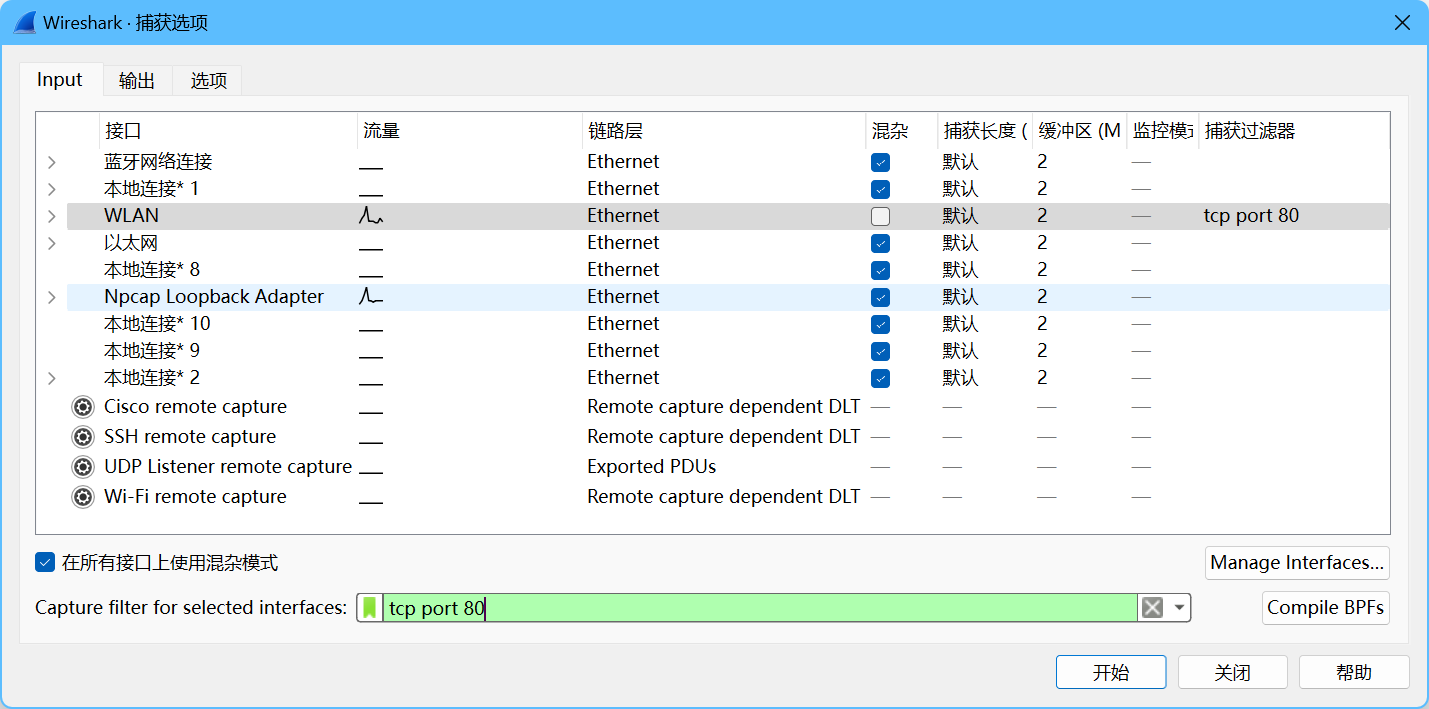
\includegraphics[width=0.8\textwidth]{img/1.png}
  \caption{设置捕获选项}
  \label{fig:1}
\end{figure}

然后,在命令行中使用\texttt{wget}命令向\texttt{http://www.baidu.com}发送\texttt{HTTP}请求。

\begin{figure}[H]
  \centering
  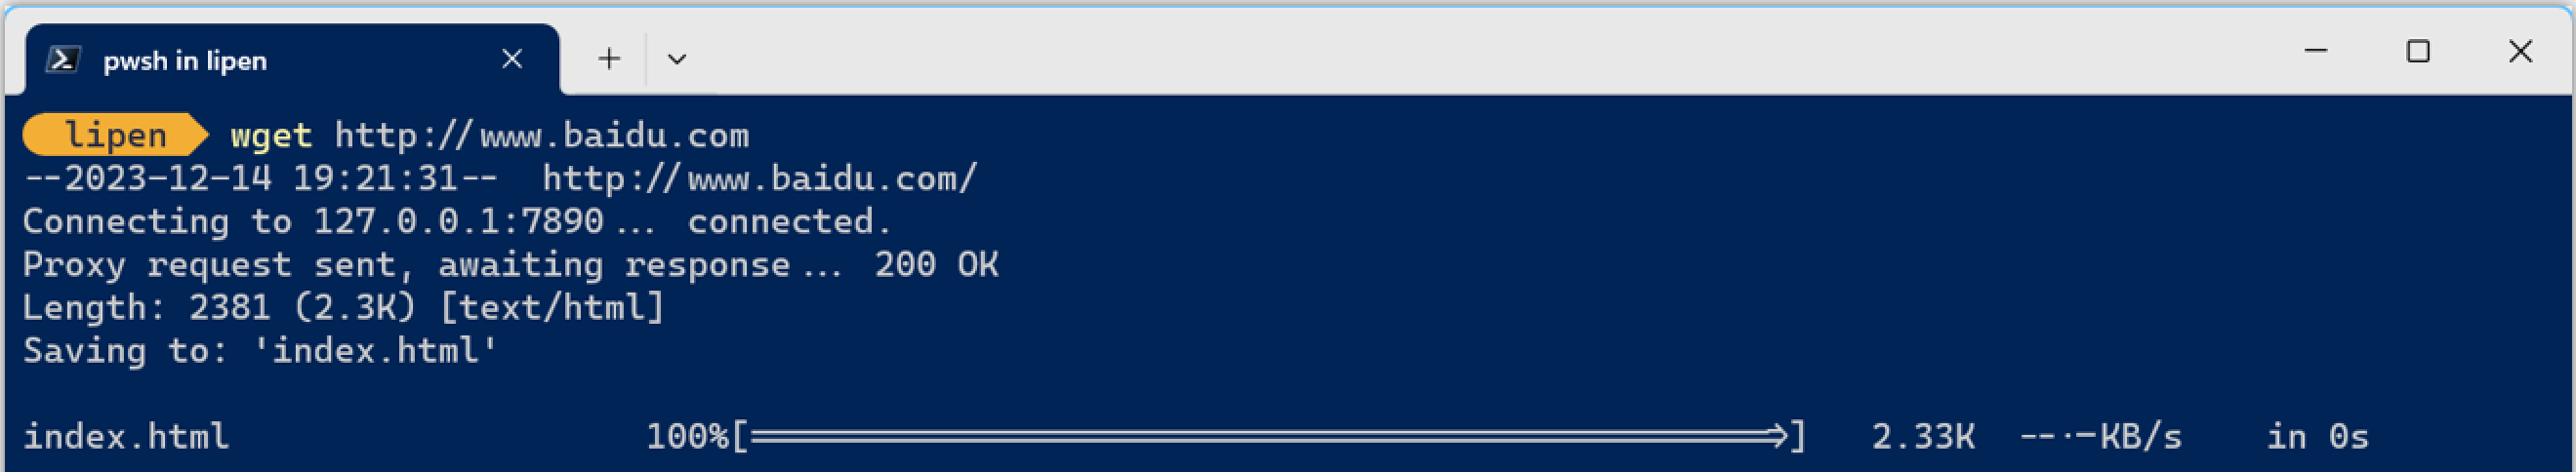
\includegraphics[width=0.8\textwidth]{img/2.png}
  \caption{使用\texttt{wget}发送\texttt{HTTP}请求}
  \label{fig:2}
\end{figure}

打开\texttt{Wireshark}的捕获窗口,停止捕获。捕获结果如下图所示:

\begin{figure}[H]
  \centering
  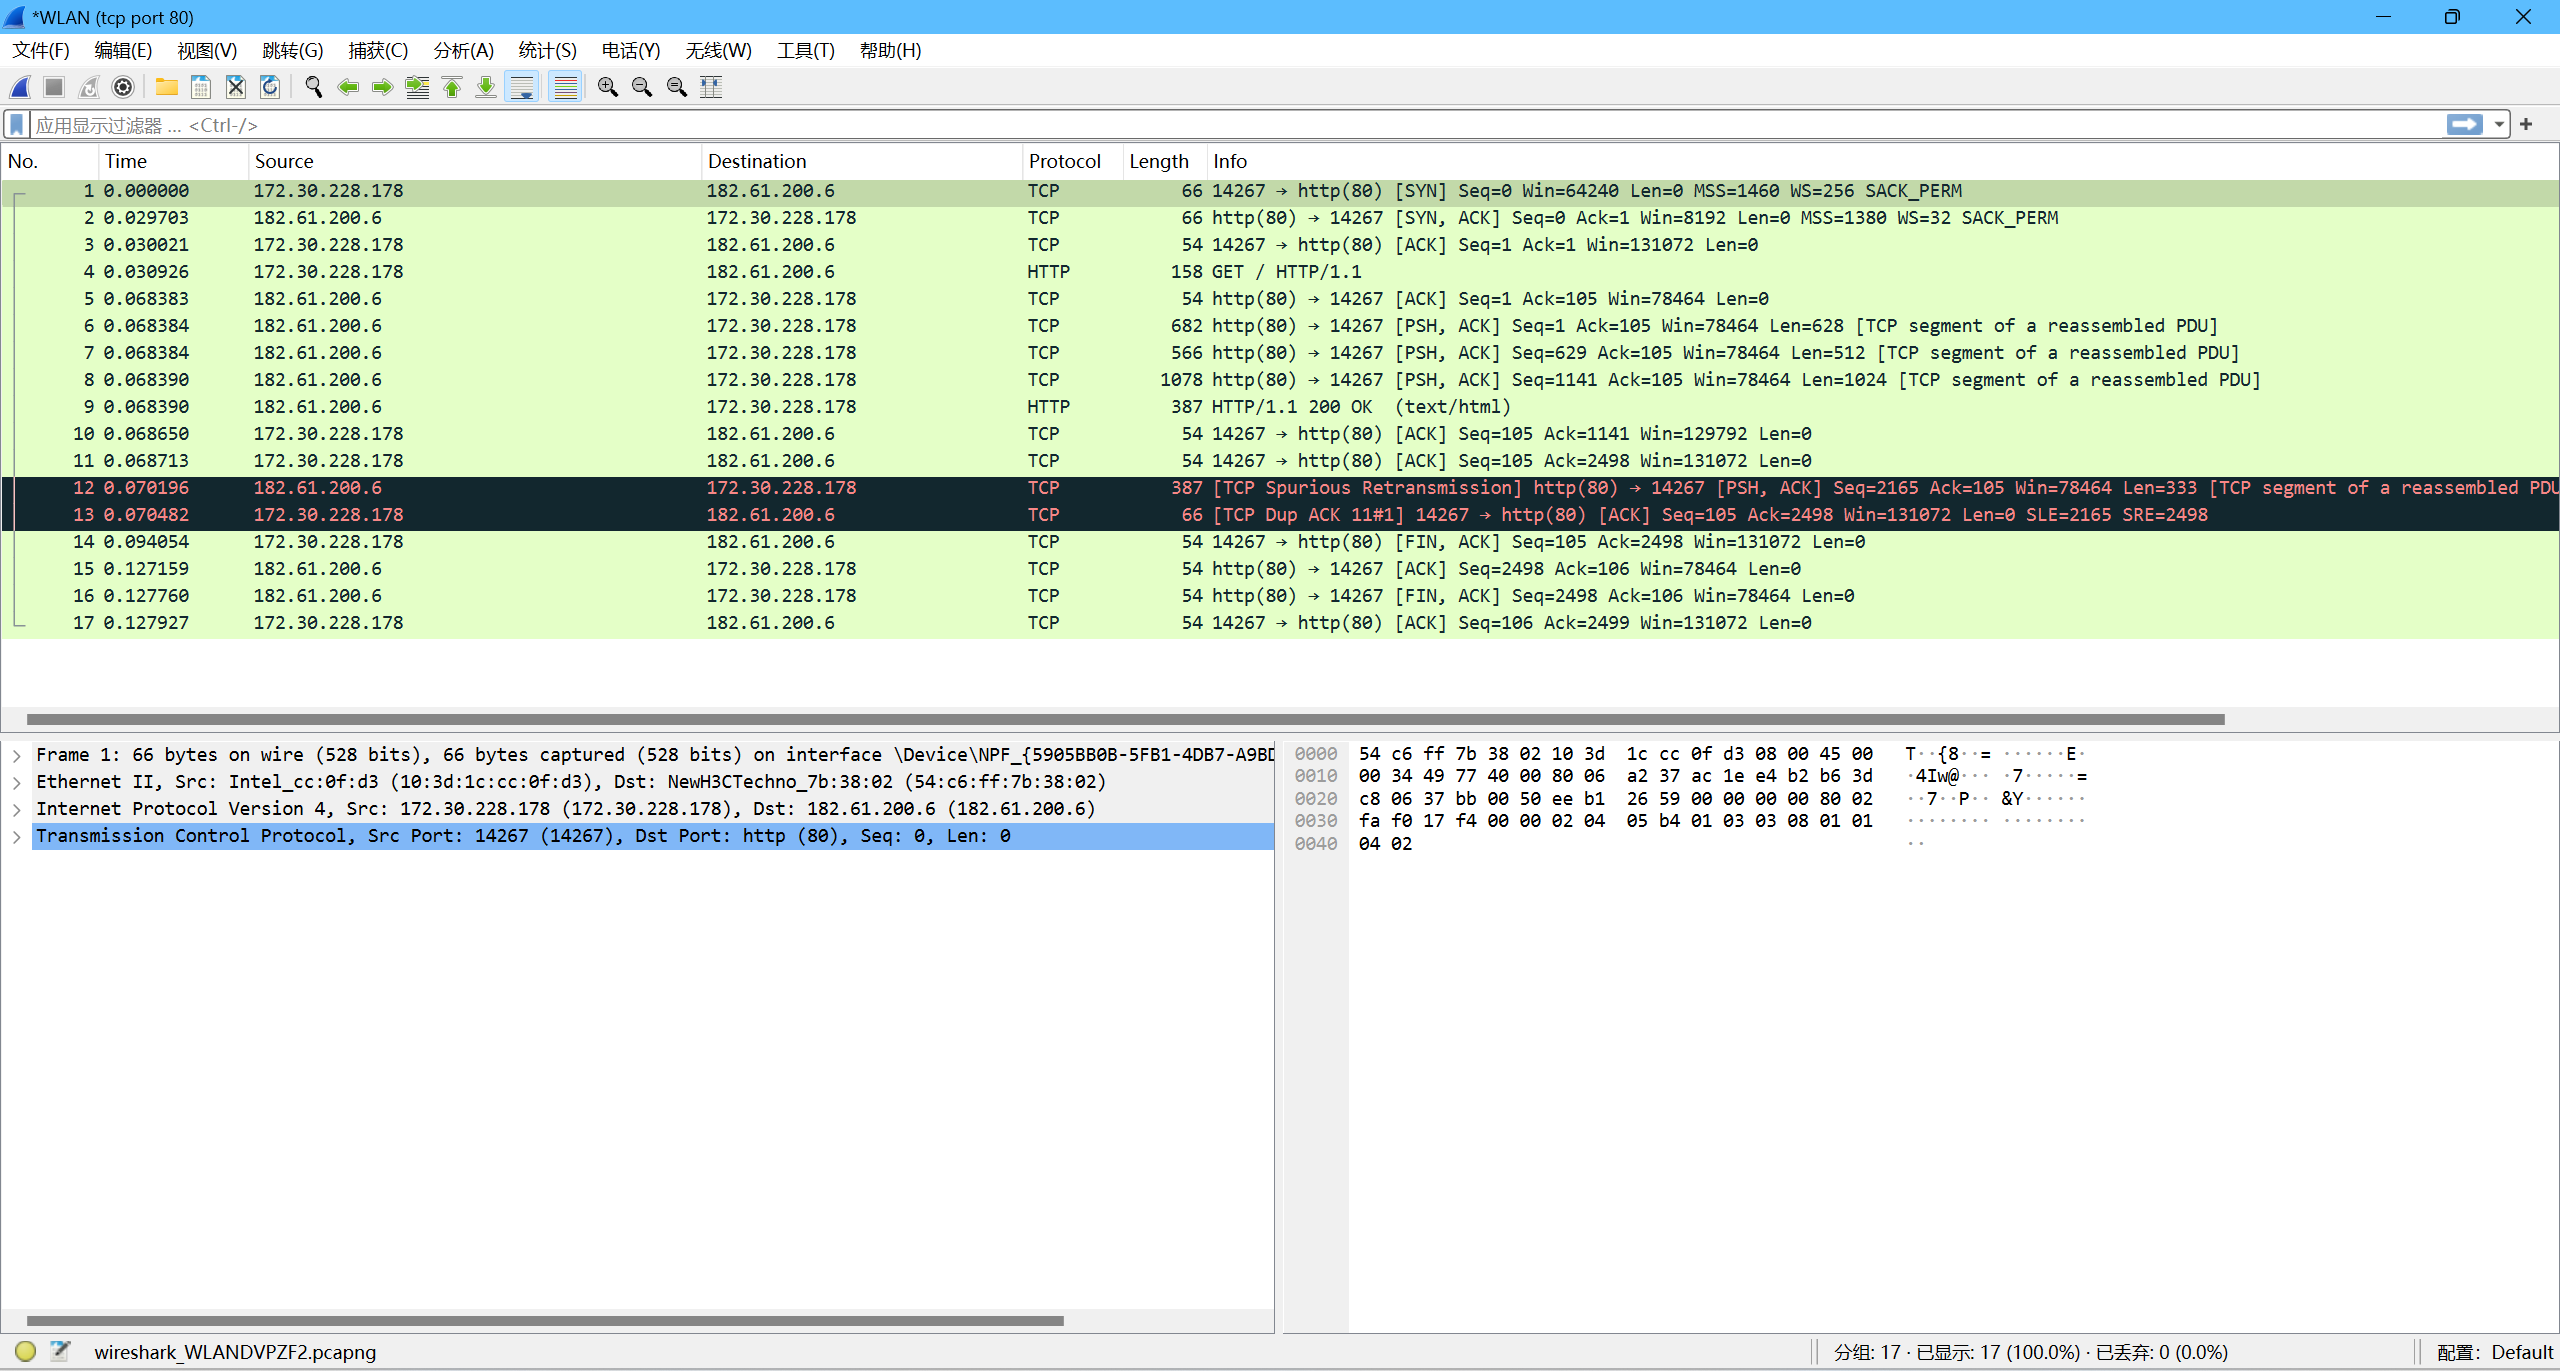
\includegraphics[width=0.8\textwidth]{img/3.png}
  \caption{捕获结果}
  \label{fig:3}
\end{figure}


\subsection{分析IPV4包并绘制报文结构 \& 数据分析}

我们选择其中的一个\texttt{IP}数据报,分析其结构,如下图所示:

\begin{figure}[H]
  \centering
  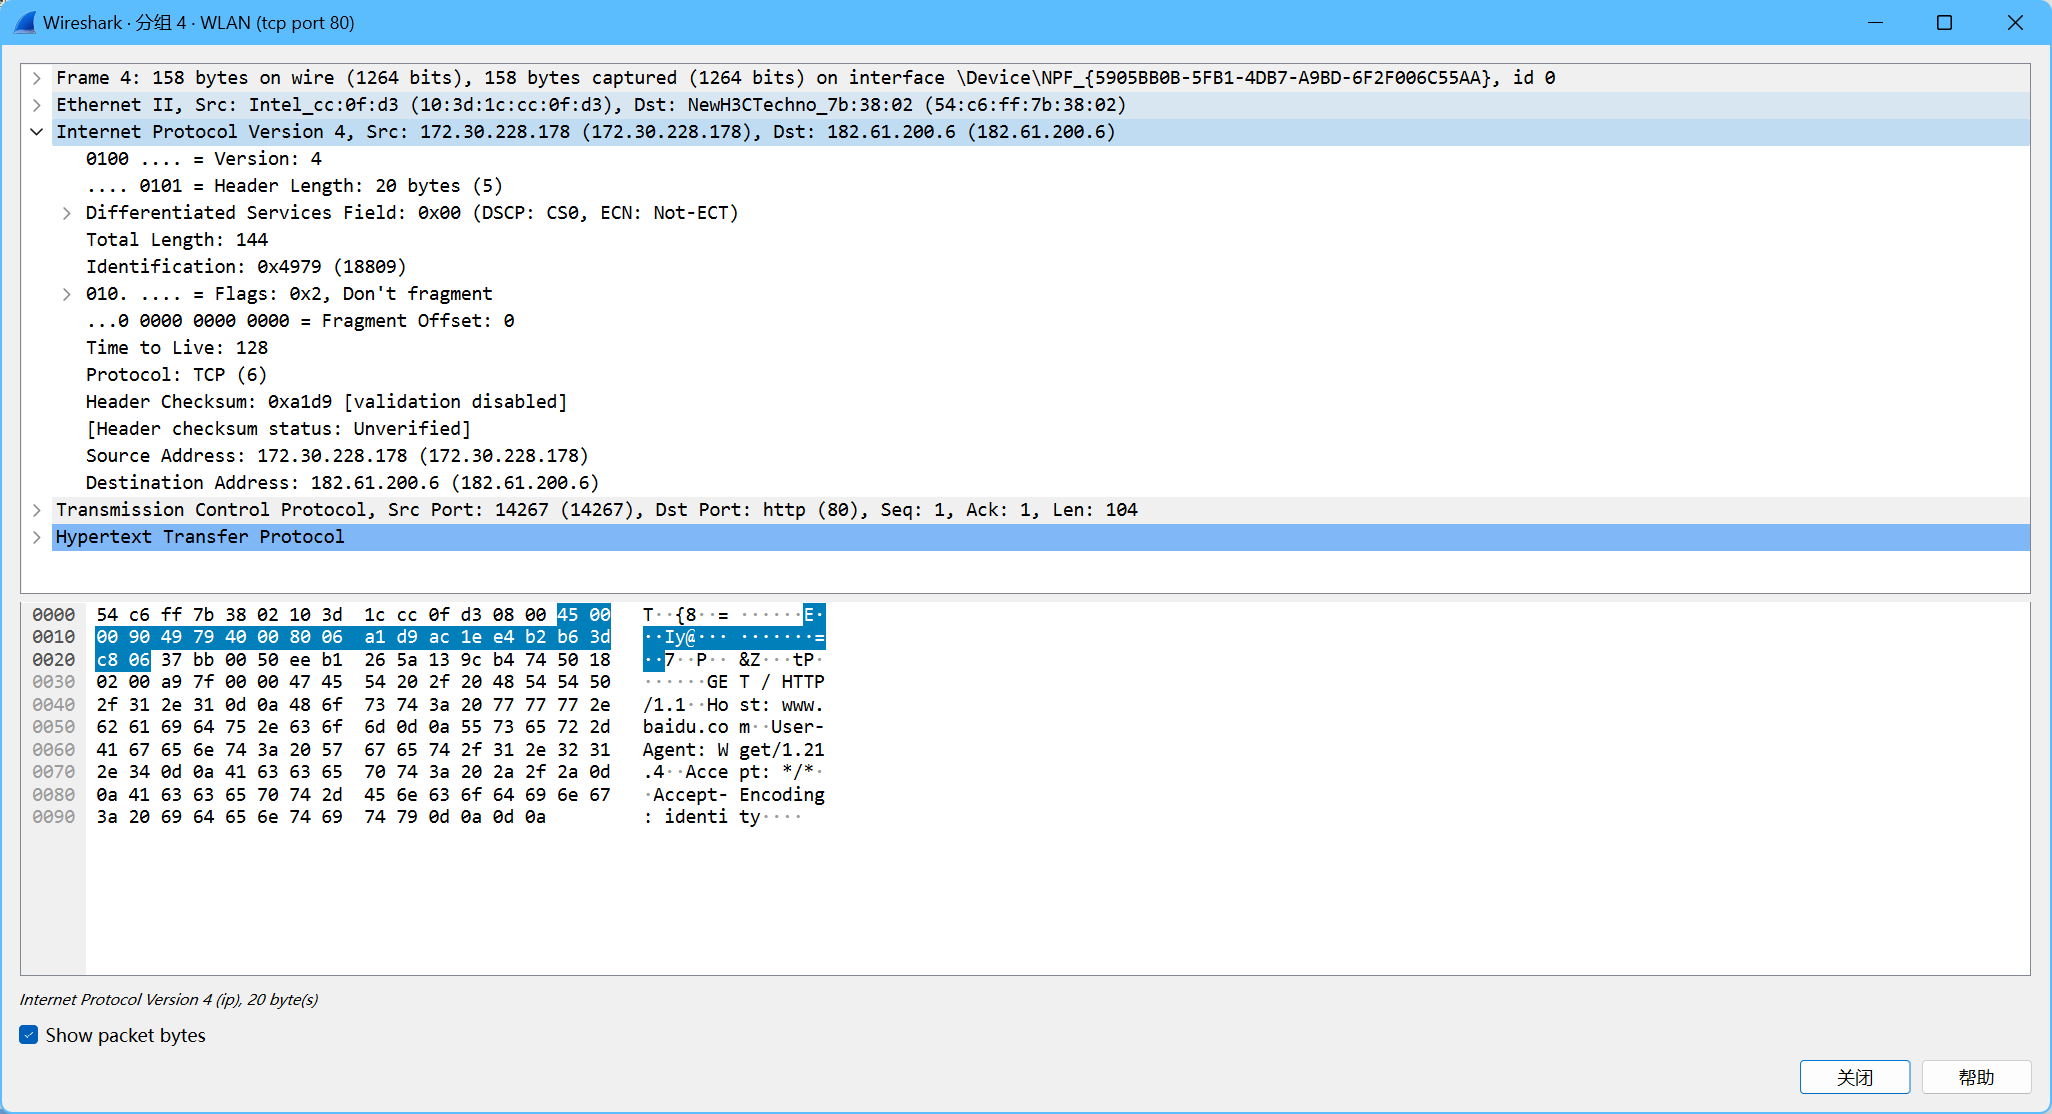
\includegraphics[width=0.8\textwidth]{img/4.png}
  \caption{\texttt{IP}数据报结构}
  \label{fig:4}
\end{figure}

可以看到,第一个字段表示版本号,长度为 \texttt{4bit},表示目前采用的IP协议的版本号。一般为\texttt{0100(IPv4)}或\texttt{0110(IPv6)}。

\begin{figure}[H]
  \centering
  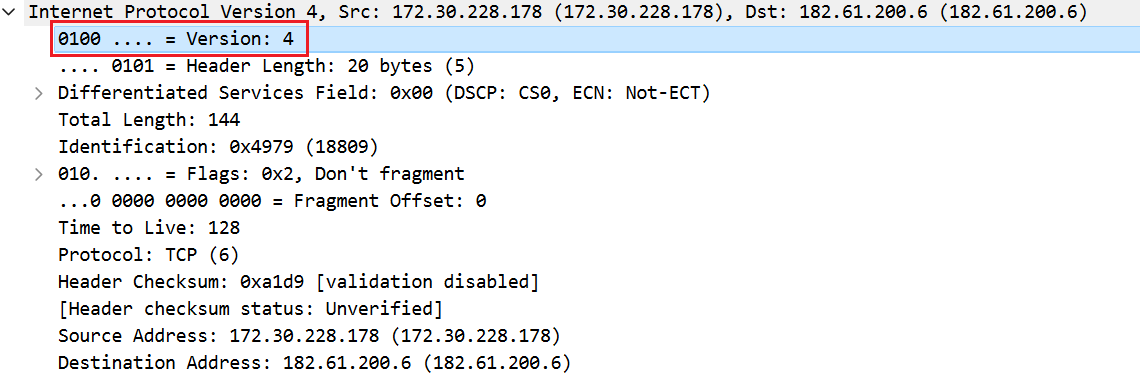
\includegraphics[width=0.8\textwidth]{img/4_1.png}
  \caption{\texttt{Version}字段}
  \label{fig:5}
\end{figure}

第二个字段表示首部长度,长度为 \texttt{4bit},表示IP报头的长度。在这个数据报中,首部长度为 \texttt{20 bytes}。

\begin{figure}[H]
  \centering
  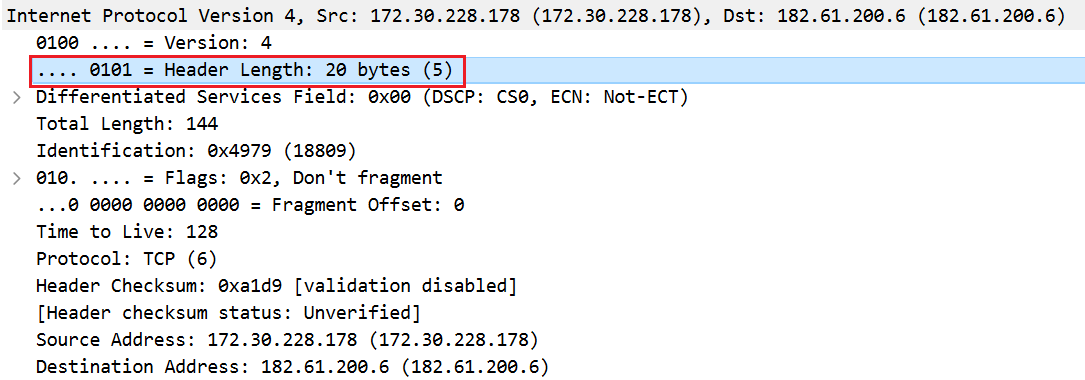
\includegraphics[width=0.8\textwidth]{img/5.png}
  \caption{\texttt{Header Length}字段}
  \label{fig:6}
\end{figure}

第三个字段表示区分服务,长度为 \texttt{1 byte},用于为不同的 \texttt{IP} 数据报定义不同的服务质量。

\begin{figure}[H]
  \centering
  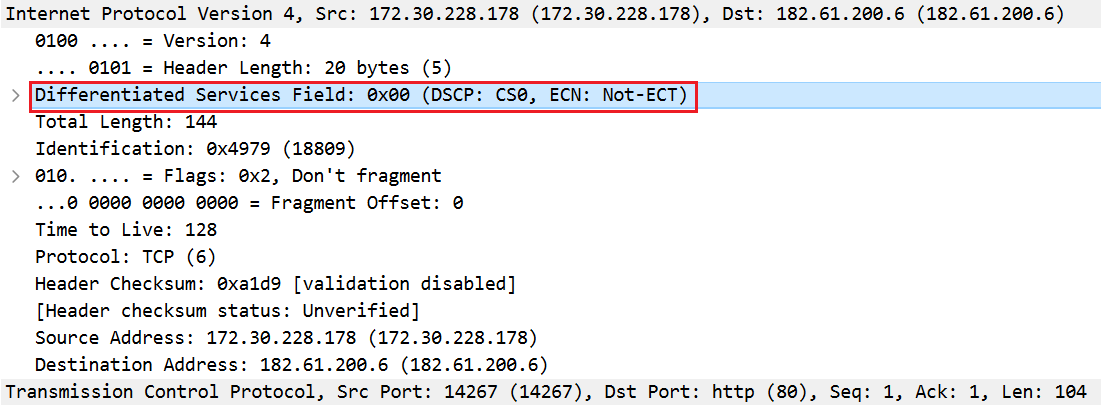
\includegraphics[width=0.8\textwidth]{img/6.png}
  \caption{\texttt{Differentiated Services}字段}
  \label{fig:7}
\end{figure}

在这个字段中,包括两个部分,第一个部分是 \texttt{DSCP},长度为 \texttt{6 bit},表示区分服务代码点,用于区分不同的服务质量。第二个部分是 \texttt{ECN},长度为 \texttt{2 bit},表示显式拥塞通知,用于指示网络拥塞。在这个数据报中, \texttt{DSCP} 的值为 \texttt{0x00},表示默认服务, \texttt{ECN} 的值为 \texttt{0x00},表示没有拥塞。

% 一行两张图片
\begin{figure}[H]
  \centering
  \begin{minipage}[t]{0.48\textwidth}
    \centering
    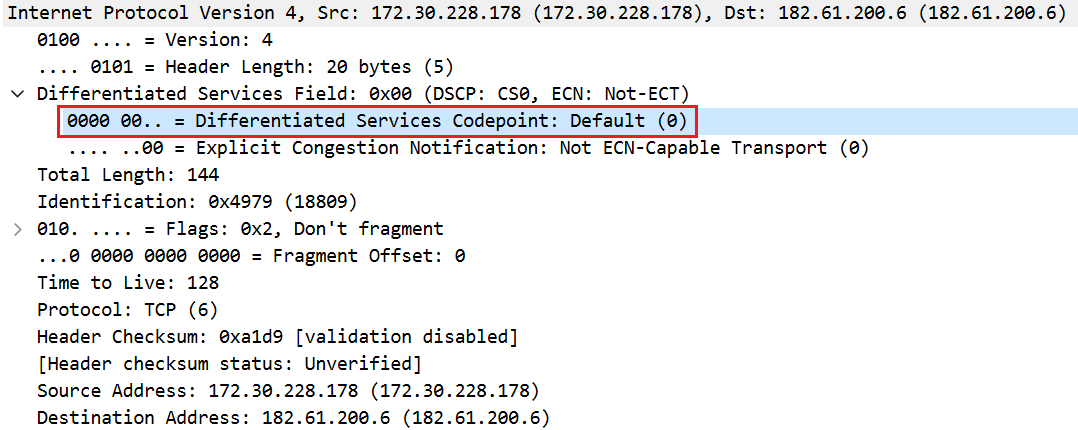
\includegraphics[width=\textwidth]{img/10.png}
    \caption{\texttt{DSCP}字段}
    \label{fig:8}
  \end{minipage}
  \begin{minipage}[t]{0.48\textwidth}
    \centering
    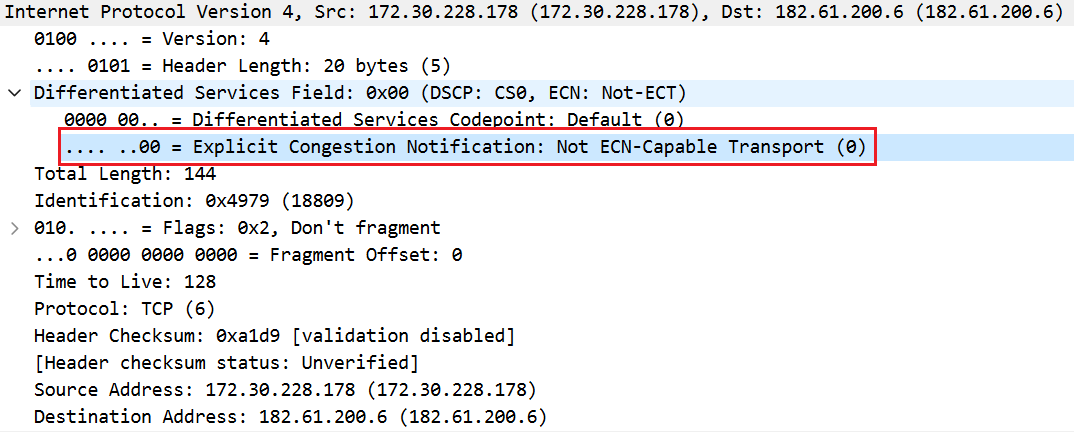
\includegraphics[width=\textwidth]{img/11.png}
    \caption{\texttt{ECN}字段}
    \label{fig:9}
  \end{minipage}
\end{figure}

第四个字段表示总长度,长度为 \texttt{2 bytes},表示以字节为单位计算的 \texttt{IP} 包的长度(包括头部和数据),所以 \texttt{IP} 包最大长度 \texttt{65 535 bytes}。数据包有效载荷的大小 = \texttt{IP} 包总长度(\texttt{Total Length})- \texttt{IP} 报头长度(\texttt{Header Length})。在这个数据报中,总长度为 \texttt{144 bytes}。


\begin{figure}[H]
  \centering
  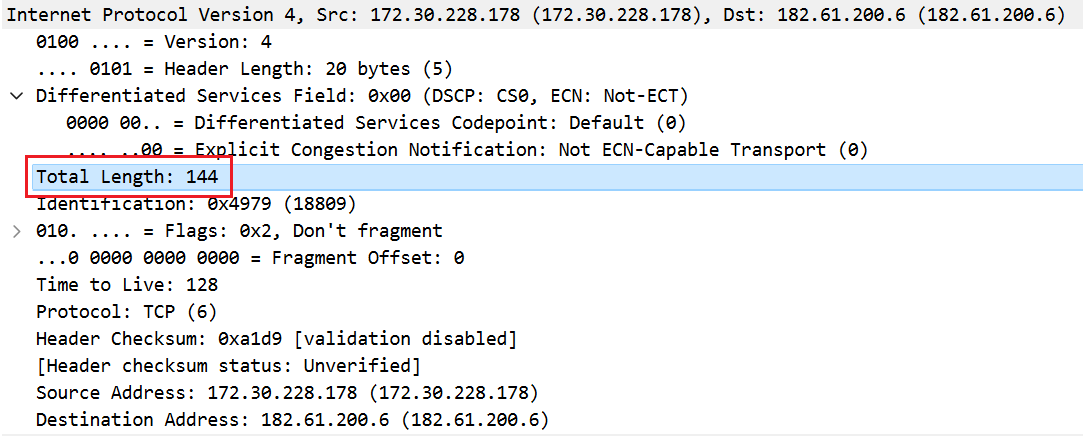
\includegraphics[width=0.6\textwidth]{img/12.png}
  \caption{\texttt{Total Length}字段}
  \label{fig:10}
\end{figure}

第五个字段为标识,长度为 \texttt{2 bytes},该字段和 \texttt{Flags} 和 \texttt{Fragment Offest} 字段联合使用,对较大的数据报进行分段(fragment)操作。路由器将一个数据报拆分后,所有拆分开的分段被标记相同的值,以便目的端设备能够区分哪个包属于被拆分开的包的一部分。在这个数据报中,标识为 \texttt{0x4979}。

\begin{figure}[H]
  \centering
  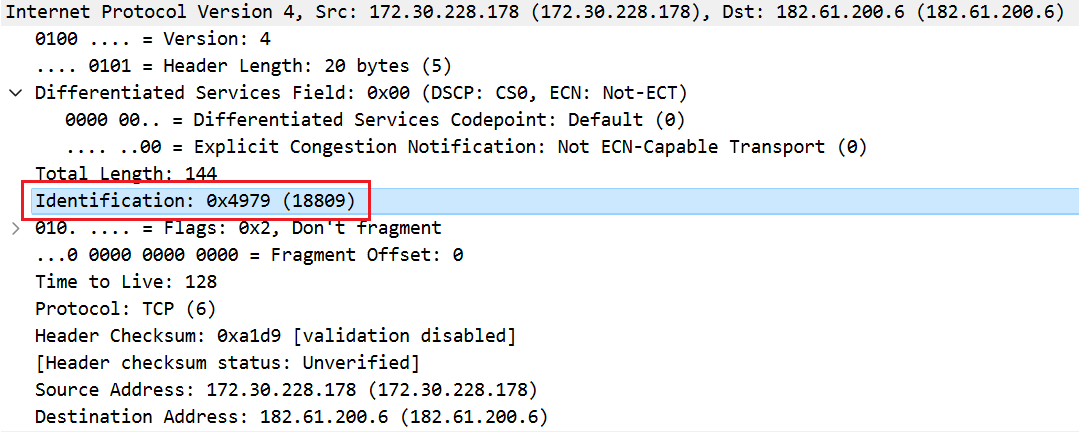
\includegraphics[width=0.6\textwidth]{img/13.png}
  \caption{\texttt{Identifier}字段}
  \label{fig:11}
\end{figure}

第六个字段为标志,长度为 \texttt{3 bit},该字段第一位不使用。第二位是 \texttt{DF(Don’t Fragment)}位, \texttt{DF = 1} 时表明路由器不能对该数据报分段。如果一个上层数据报无法在不分段的情况下进行转发,则路由器会丢弃该上层数据包并返回一个错误信息。第三位是 \texttt{MF(More Fragments)}位, \texttt{MF=1} 表示后面还有分片的数据报, \texttt{MF=0} 表示这已经是若干数据报片中的最后一个。在这个数据报中,标志为 \texttt{0x02},表示不分段,且后面没有分片的数据报。

\begin{figure}[H]
  \centering
  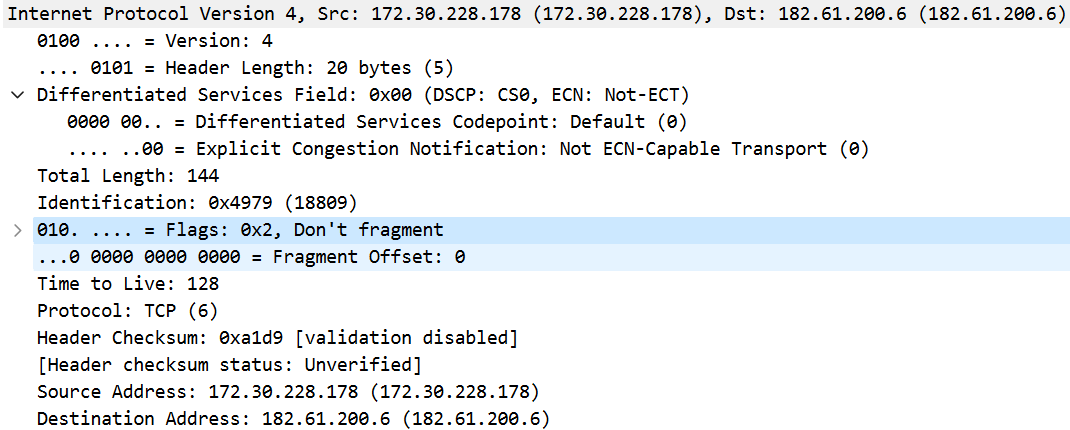
\includegraphics[width=0.8\textwidth]{img/14.png}
  \caption{\texttt{Flags}字段}
  \label{fig:12}
\end{figure}

\begin{figure}[H]
  \centering
  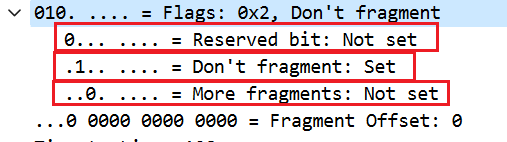
\includegraphics[width=0.8\textwidth]{img/15.png}
  \caption{\texttt{Flags}字段内容}
  \label{fig:13}
\end{figure}

第七个字段为片偏移,长度为 \texttt{13 bit},以 \texttt{8} 个字节为偏移单位。 片偏移量用来告诉接收端这个分片在原数据报的相对位置,相对于原数据报的数据部分,该分片从何处开始,是开始还是中间,以便于进行重组还原 \texttt{IP} 包。在这个数据报中,片偏移为 \texttt{0}。

\begin{figure}[H]
  \centering
  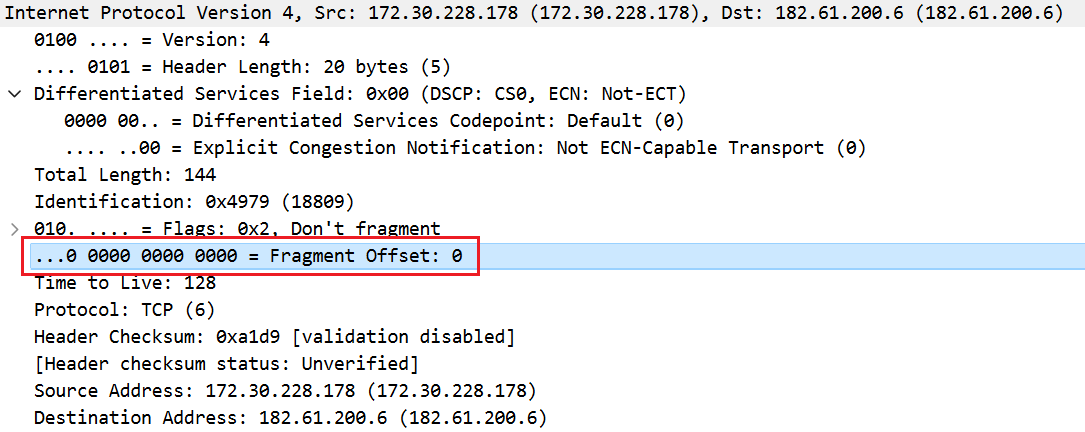
\includegraphics[width=0.8\textwidth]{img/15_2.png}
  \caption{\texttt{Fragment Offset}字段}
  \label{fig:14}
\end{figure}

第八个字段为生存时间,长度为 \texttt{8 bit},以跳数为单位。用以表明数据报文在网络传输过程中能经过的跳数。根据操作系统不同,TTL默认值不同,每经过一个三层设备如路由器的处理,TTL值会减去1,当TTL=0的时候,此数据报就会被丢弃。这个字段可以防止由于路由环路而导致 \texttt{IP} 包在网络中不停被转发。在这个数据报中,生存时间为 \texttt{128}。

\begin{figure}[H]
  \centering
  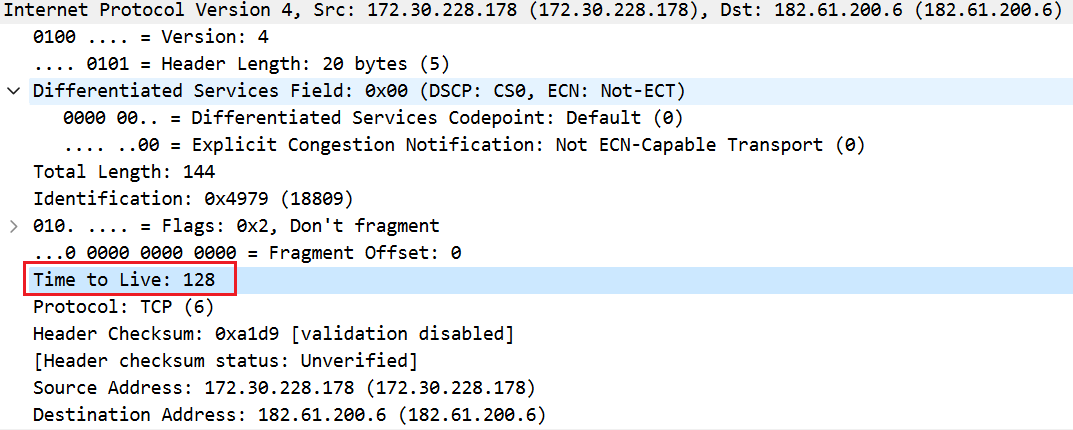
\includegraphics[width=0.8\textwidth]{img/16.png}
  \caption{\texttt{TTL}字段}
  \label{fig:15}
\end{figure}

第九个字段为协议,长度为 \texttt{8 bit}。标识了上层所使用的协议。在这个数据报中,协议为 \texttt{TCP},值为 \texttt{0x06}。

\begin{figure}[H]
  \centering
  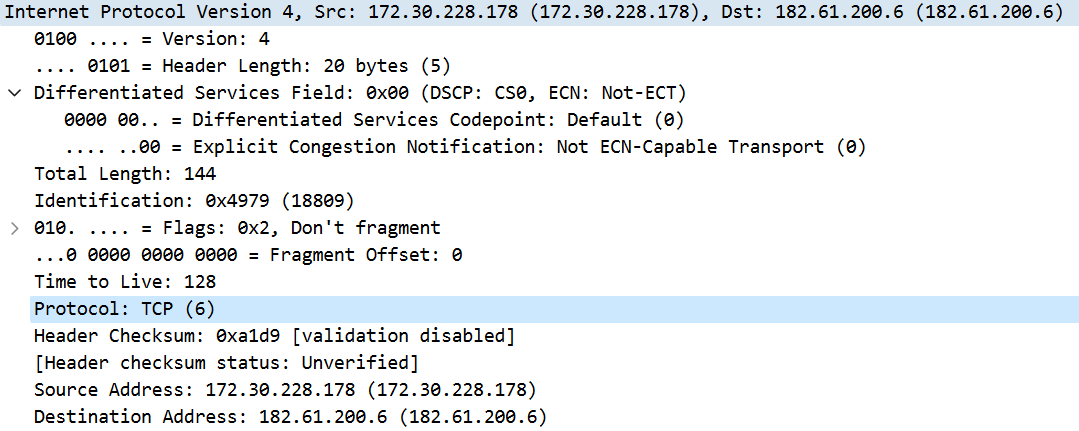
\includegraphics[width=0.8\textwidth]{img/17.png}
  \caption{\texttt{Protocol}字段}
  \label{fig:16}
\end{figure}

第十个字段为首部校验和,长度为 \texttt{16 bit}。用来做 \texttt{IP} 头部的正确性检测,但不包含数据部分。在这个数据报中,首部校验和为 \texttt{0xa1d9}。

\begin{figure}[H]
  \centering
  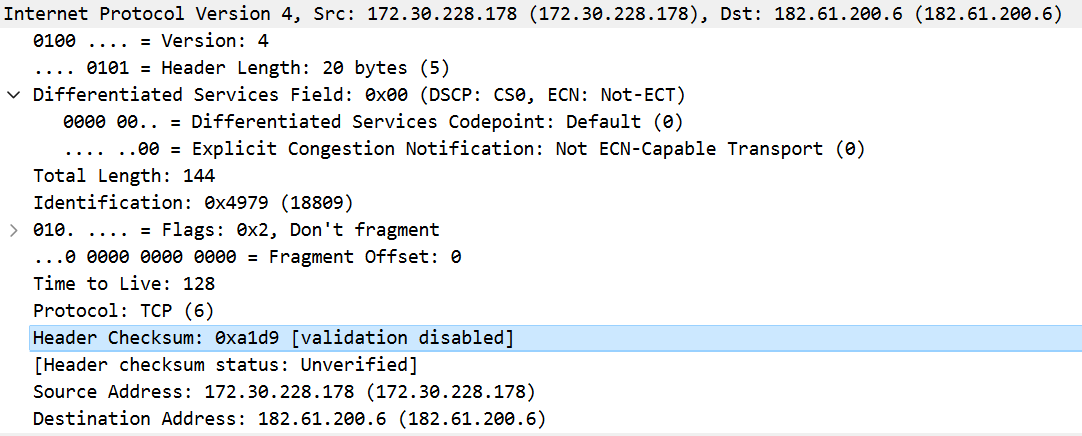
\includegraphics[width=0.8\textwidth]{img/18.png}
  \caption{\texttt{Header Checksum}字段}
  \label{fig:17}
\end{figure}

第十一个字段为源IP地址,长度为 \texttt{32 bit},表示发送方的IP地址。在这个数据报中,源IP地址为 \texttt{172.30.228.178}

\begin{figure}[H]
  \centering
  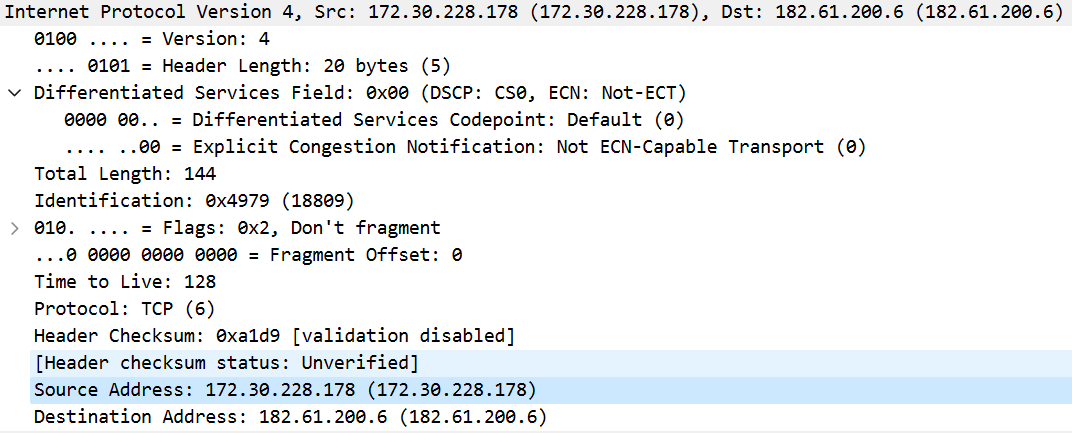
\includegraphics[width=0.8\textwidth]{img/19.png}
  \caption{\texttt{Source Address}字段}
  \label{fig:18}
\end{figure}

第十二个字段为目的IP地址,长度为 \texttt{32 bit},表示接收方的IP地址。在这个数据报中,目的IP地址为 \texttt{182.61.200.6}

\begin{figure}[H]
  \centering
  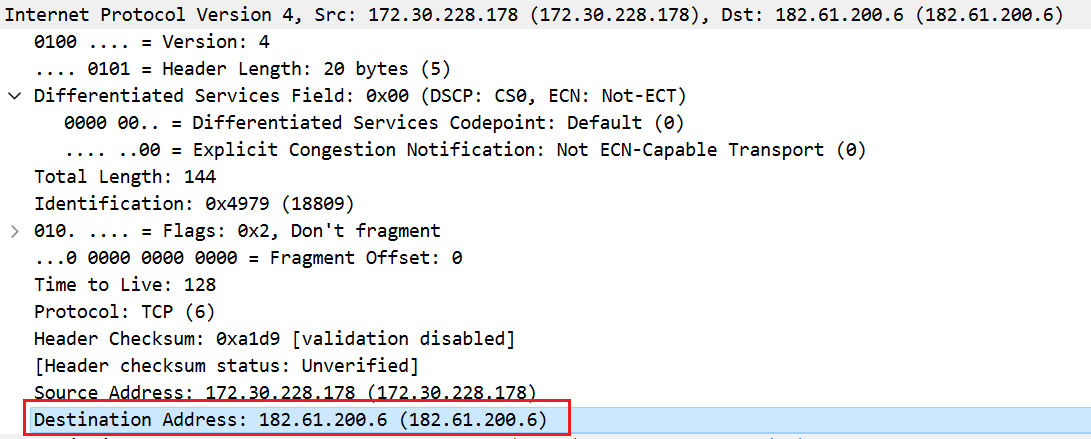
\includegraphics[width=0.8\textwidth]{img/20.png}
  \caption{\texttt{Destination Address}字段}
  \label{fig:19}
\end{figure}

\textbf{可以做出如下示意图来表示 \texttt{IP} 数据报的结构:}

\begin{figure}[H]
  \centering
  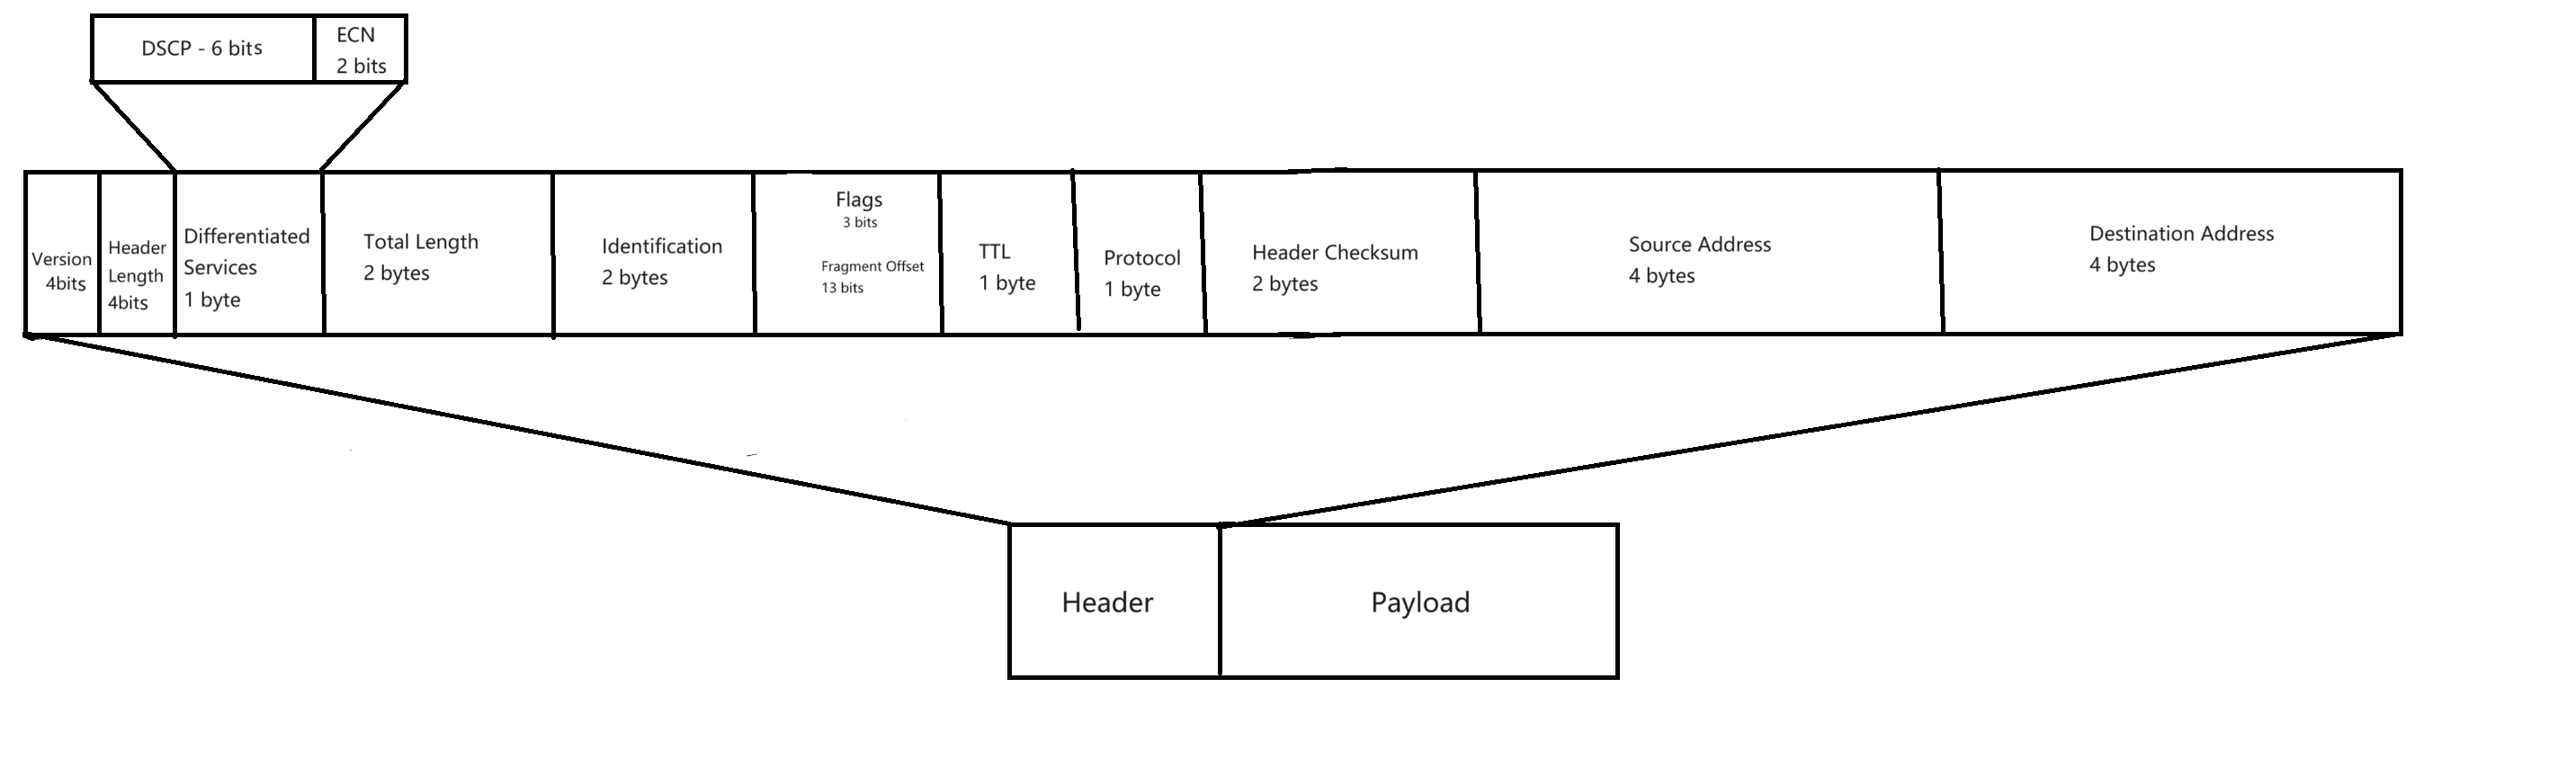
\includegraphics[width=0.9\textwidth]{img/21.png}
  \caption{\texttt{IP}数据报结构示意图}
  \label{fig:20}
\end{figure}

\subsection{回答问题}

\begin{enumerate}[noitemsep]
  \item 你的计算机和远程服务器的IP地址是什么? 

        \textbf{答:}我的电脑的IP地址为 \texttt{172.30.228.178},远程服务器的IP地址为 \texttt{182.61.200.6}。
  \item “总长度”字段是否包括IP报头加上IP有效负载,或者仅包括IP有效负载?

        \textbf{答:}\texttt{Total Length}字段包括\texttt{IP}报头和\texttt{IP}数据的总长度。
  \item 对于不同的数据包,“标识”字段的值如何变化,还是保持不变? 例如,对于TCP连接中的所有数据包,它一直保持相同的值,还是对于每个数据包都不同? 双向通信的报文是否相同? 如果值发生变化,您能看到任何规律吗?

        \textbf{答:}标识字段的值在不同的数据包中不同。在同一个 \texttt{TCP}连接中,标识字段的值不同。在同一个方向上,标识字段的值不同。在不同的方向上,标识字段的值不同。在这个数据报中,标识字段的值为 \texttt{0x4979}。
  \item 从您的计算机发送的数据包的TTL字段的初始值是多少?他们是maximum possible value吗?

        \textbf{答:}我的电脑发送的数据包的生存时间字段的初始值为 \texttt{128},不是最大值。
  \item 查看数据包时如何判断它是否被分段?

        \textbf{答:}如果一个数据包没有被分段,那么它的标志字段的 \texttt{DF}位为 \texttt{1},且标志字段的 \texttt{MF}位为 \texttt{0}。
  \item IP数据报报头的长度是多少,它是如何被编码进报头长度域的?

        \textbf{答:}\texttt{IP}报头的长度为 \texttt{20 bytes},版本号和首部长度字段共占 \texttt{8 bits},其中版本号占 \texttt{4 bits},首部长度占 \texttt{4 bits}。
\end{enumerate}

\subsection{traceroute结果分析}

在命令行下使用tracert命令,查看到达\texttt{www.baidu.com}的路由路径。根据输出画出网络路径。(实验地点有所差别,顾目标IP地址略有不同)

\begin{figure}[H]
  \centering
  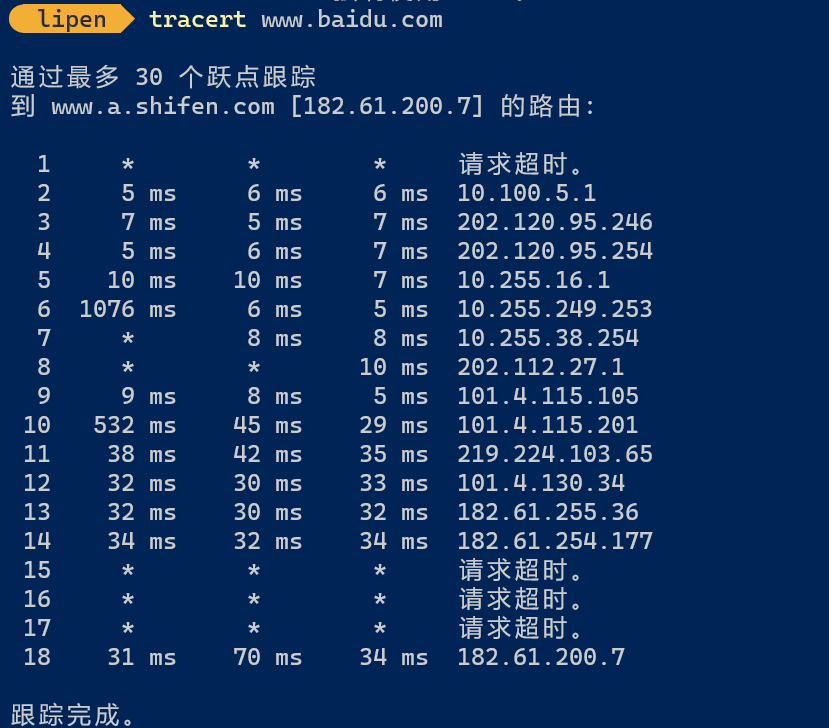
\includegraphics[width=0.8\textwidth]{img/22.png}
  \caption{\texttt{tracert}命令输出}
  \label{fig:21}
\end{figure}

画出网络路径图如下:

\begin{figure}[H]
  \centering
  \begin{tikzpicture}[node distance=0.5cm, >=Stealth, rect/.style={draw, minimum width=2cm, minimum height=1cm, text centered}]

    % Draw rectangles
    \node (me) [rect] {本机};
    \node (1) [rect, below=of me] {*};
    \node (2) [rect, below=of 1] {10.100.5.1};
    \node (3) [rect, below=of 2] {202.120.95.246};
    \node (4) [rect, below=of 3] {202.120.95.254};
    \node (5) [rect, below=of 4] {10.255.16.1};
    \node (6) [rect, below=of 5] {10.255.249.253};
    \node (7) [rect, below=of 6] {10.255.38.254};
    \node (8) [rect, below=of 7] {202.112.27.1};
    \node (9) [rect, below=of 8] {101.4.115.105};
    \node (10) [rect, right=of 9] {101.4.115.201};
    \node (11) [rect, above=of 10] {219.224.103.65};
    \node (12) [rect, above=of 11] {101.4.130.34};
    \node (13) [rect, above=of 12] {182.61.255.36};
    \node (14) [rect, above=of 13] {182.61.254.177};
    \node (15) [rect, above=of 14] {*};
    \node (16) [rect, above=of 15] {*};
    \node (17) [rect, above=of 16] {*};
    \node (18) [rect, above=of 17] {182.61.200.7};

    % Draw arrows
    \draw[->] (me.south) -- (1.north);
    \draw[->] (1.south) -- (2.north);
    \draw[->] (2.south) -- (3.north);
    \draw[->] (3.south) -- (4.north);
    \draw[->] (4.south) -- (5.north);
    \draw[->] (5.south) -- (6.north);
    \draw[->] (6.south) -- (7.north);
    \draw[->] (7.south) -- (8.north);
    \draw[->] (8.south) -- (9.north);
    \draw[->] (9.east) -- (10.west);
    \draw[->] (10.north) -- (11.south);
    \draw[->] (11.north) -- (12.south);
    \draw[->] (12.north) -- (13.south);
    \draw[->] (13.north) -- (14.south);
    \draw[->] (14.north) -- (15.south);
    \draw[->] (15.north) -- (16.south);
    \draw[->] (16.north) -- (17.south);
    \draw[->] (17.north) -- (18.south);



  \end{tikzpicture}
  \caption{网络路径图}
  \label{fig:22}
\end{figure}

\subsection{观察、计算IP报文的\texttt{checksum}校验和}

\texttt{IP}报头的校验和可以用来验证一个数据包是否正确。
我们选择刚才的 \texttt{IP}报文,计算它的 \texttt{checksum}。

将其校验和字段置为0后,数据如下:
45 00 00 90 49 79 40 00 80 06 00 00 ac 1e e4 b2 b6 3d c8 06

将其分为两个字节一组,进行二进制求和,再将最高位的进位加到低16位,得到的结果如下:

\begin{lstlisting}[numbers=none]
     45 00 
+    00 90 
+    49 79 
+    40 00 
+    80 06 
+    00 00 
+    ac 1e 
+    e4 b2 
+    b6 3d 
+    c8 06
--------------
   4 5e 22
+        4
--------------
     5e 26
\end{lstlisting}

取反后,得到 \texttt{checksum}为 \texttt{0xa1d9},与原数据报中的 \texttt{checksum}字段相同。

\begin{lstlisting}[numbers=none]
  ff ff
- 5e 26
-----------
  a1 d9
\end{lstlisting}

\subsection{问题讨论}

\begin{enumerate}[noitemsep]
  \item 了解并尝试使用IPv6。 现代操作系统已经包含对IPv6的支持,因此您可能能够捕获网络上的IPv6流量。 您还可以通过tunnels连接到IPv6

        \texttt{IPv6}是\texttt{IP}协议的下一代协议,它的主要特点是地址空间更大,报头更简单,安全性更好,支持多播和组播,支持流量标签,支持流量优先级,支持更多的选项和扩展,支持更多的协议。现代操作系统已经支持\texttt{IPv6},可以在网络上捕获\texttt{IPv6}流量。也可以通过隧道连接到\texttt{IPv6}提供者。

        我们使用 \texttt{Wireshark}捕获\texttt{IPv6}数据包.

        在 \texttt{Wireshark}的筛选器中输入 \texttt{ipv6},可以看到捕获到的\texttt{IPv6}数据包。

        \begin{figure}[H]
          \centering
          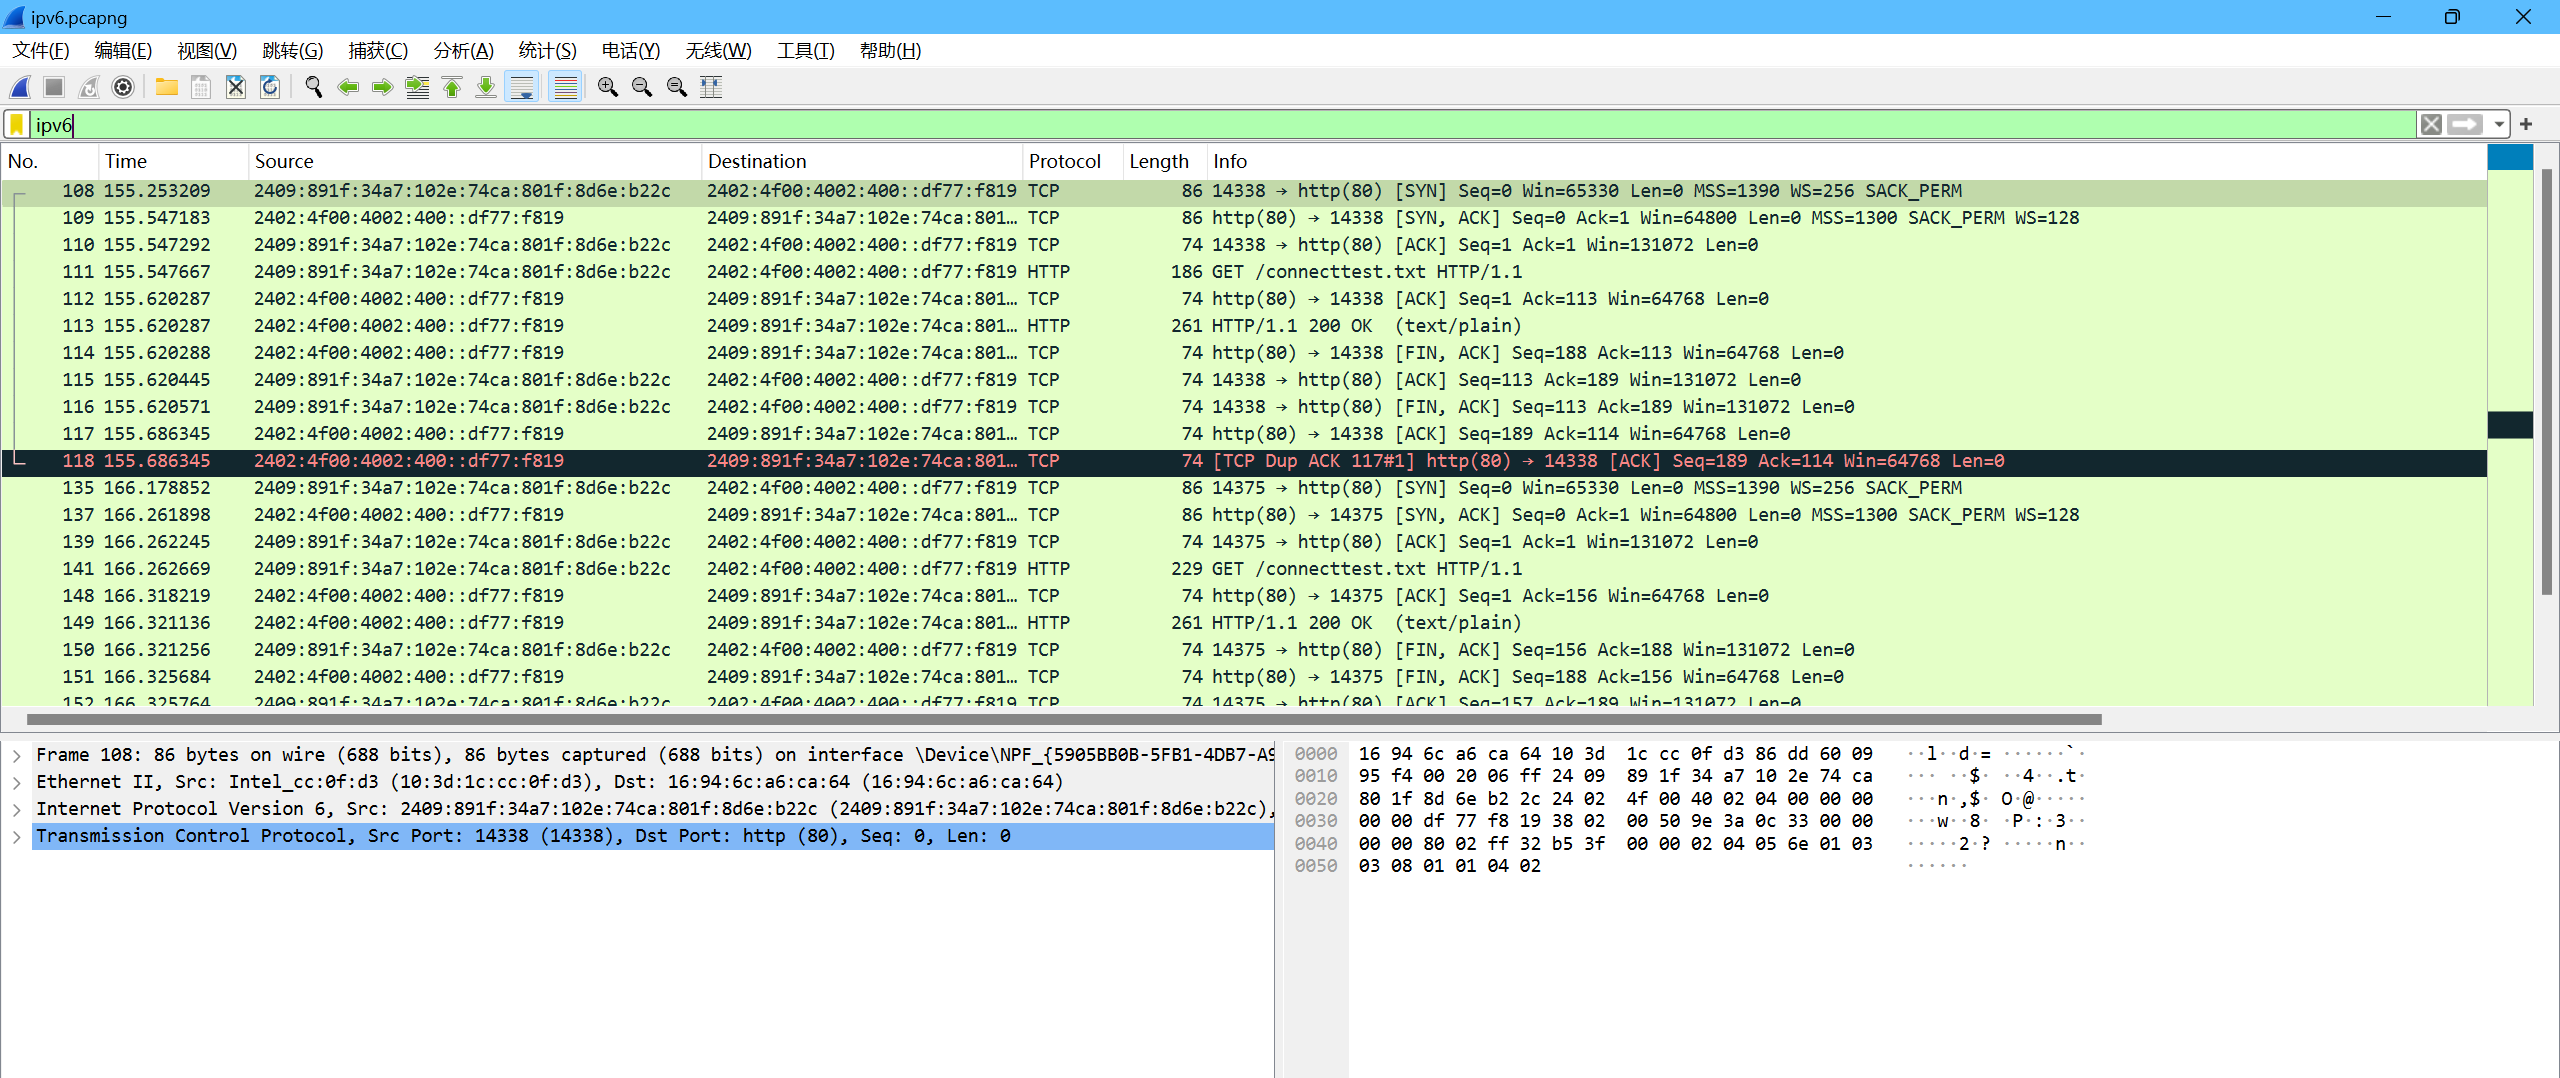
\includegraphics[width=0.8\textwidth]{img/23.png}
          \caption{\texttt{Wireshark}捕获\texttt{IPv6}数据包}
          \label{fig:23}
        \end{figure}

        选择其中的一个数据包,可以看到其结构如下:

        \begin{figure}[H]
          \centering
          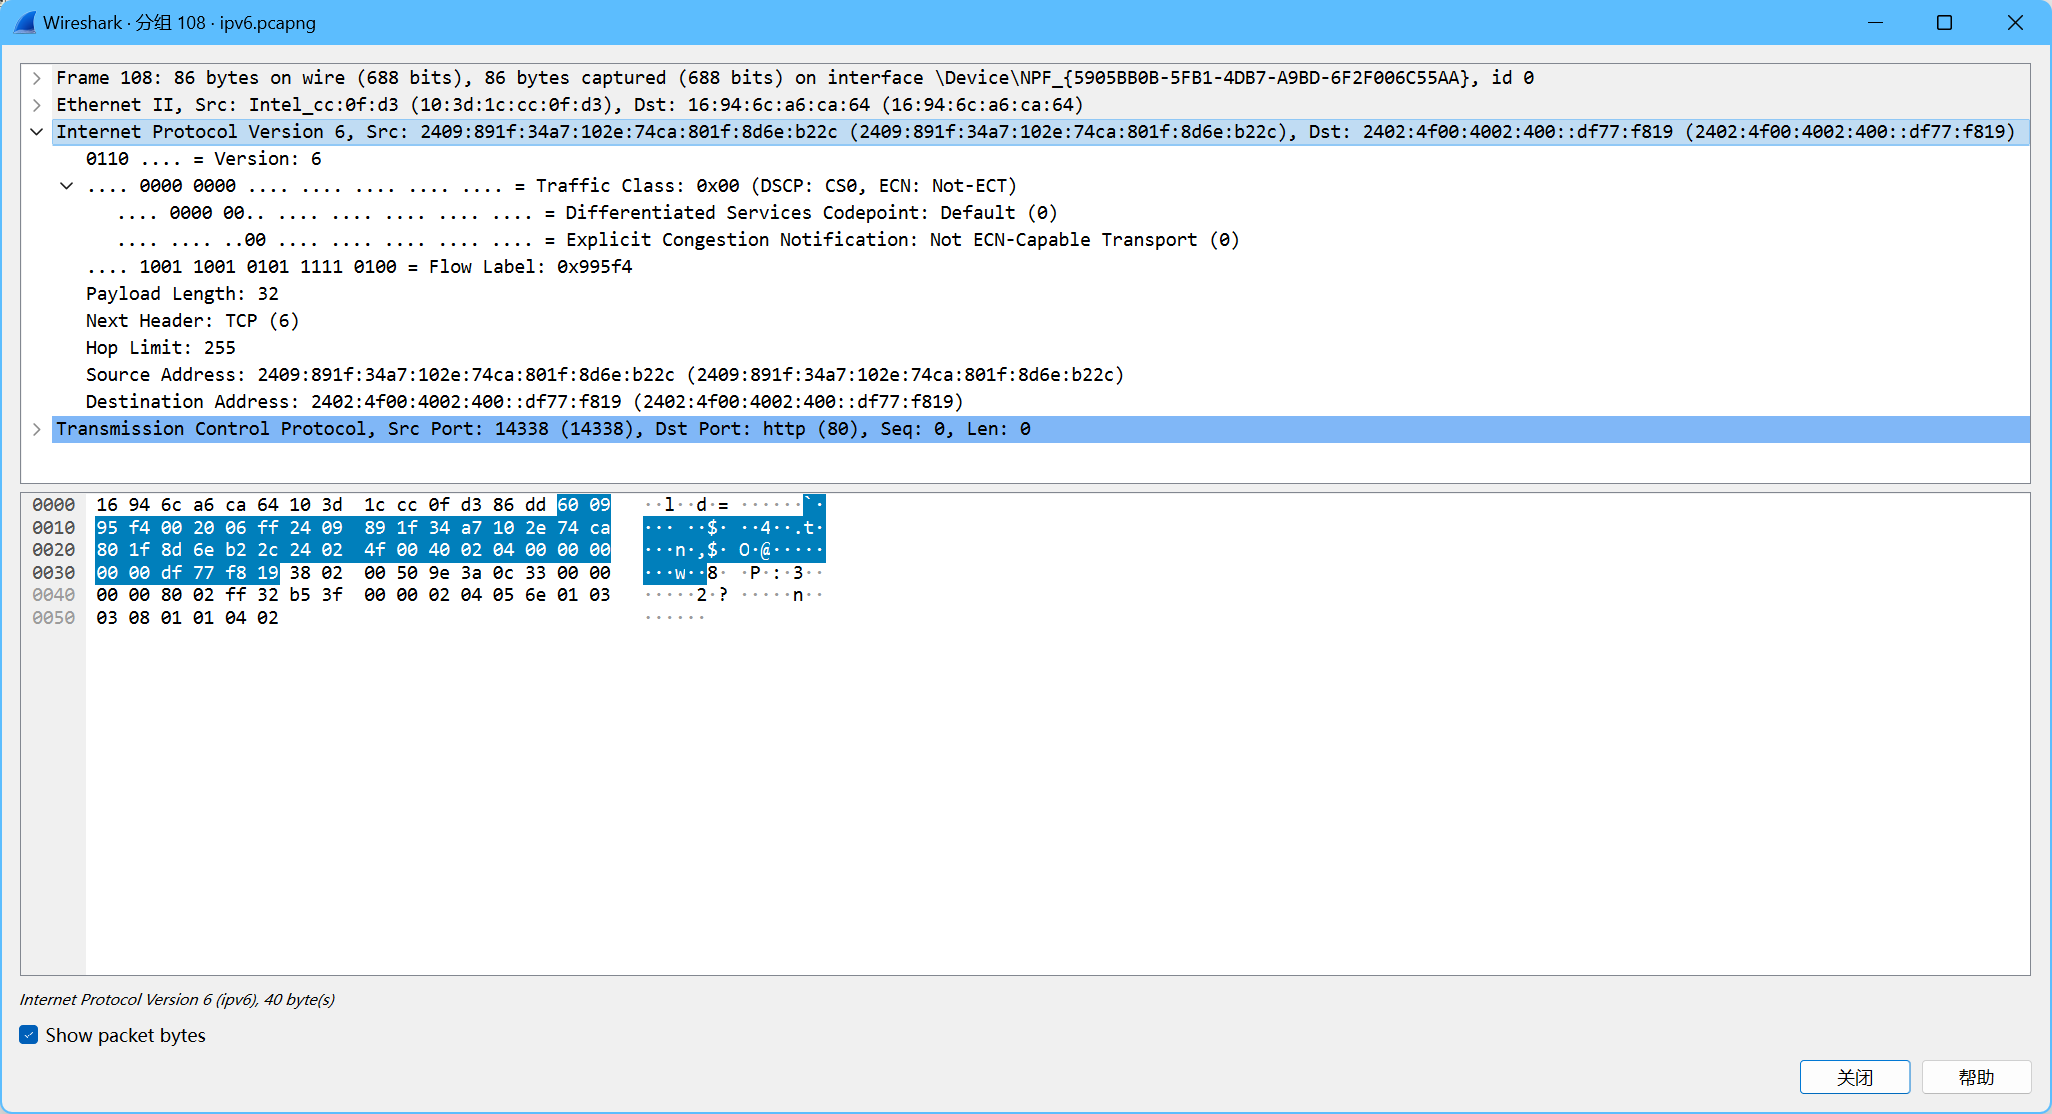
\includegraphics[width=0.8\textwidth]{img/24.png}
          \caption{\texttt{IPv6}数据包结构}
          \label{fig:24}
        \end{figure}

        可以发现,\texttt{IPv6}数据包的结构与\texttt{IPv4}数据包的结构有所不同。其中,\texttt{IPv6}数据包的首部长度为 \texttt{40 bytes},地址均为 \texttt{16 bytes},校验和字段被取消。增加了 \texttt{Hop Limit}字段,用于替代\texttt{IPv4}中的\texttt{TTL}字段。

  \item 了解tunnels技术。

        隧道是一种将一个\texttt{IP}数据包封装在另一个\texttt{IP}报头中的方法。隧道可以用于将\texttt{IPv6}数据包封装在\texttt{IPv4}数据包中,也可以用于将\texttt{IPv4}数据包封装在\texttt{IPv6}数据包中。

  \item 了解有关IP的地理位置信息,即IP地址和它对应的地理位置之间的信息。

        \texttt{IP}地理定位是将地理位置分配给\texttt{IP}地址的过程,可以使用测量或来自其名称管理数据库的线索。可以尝试使用\texttt{IP}地理定位服务。例如,\texttt{https://www.iplocation.net/} 可以根据\texttt{IP}地址查询其地理位置。

  \item 了解IPsec或IP security。 它为IP数据包提供机密性和身份验证,通常用作VPN的一部分。

        \texttt{IPsec}或\texttt{IP}安全是一种为\texttt{IP}数据包提供机密性和身份验证的协议,通常作为VPN的一部分使用。它提供了一种在网络层对数据包进行安全处理的方式,确保在传输过程中数据的机密性和完整性,并验证通信的参与方身份。
\end{enumerate}

\section{实验结果总结}

本次实验中,我们使用\texttt{Wireshark}捕获\texttt{IP}数据包,并对其进行分析。我们分析了\texttt{IP}数据包的结构,回答了相关问题。我们使用\texttt{tracert}命令查看了到达\texttt{www.baidu.com}的路由路径,并画出了网络路径图。我们选择了一个\texttt{IP}数据包,计算了其\texttt{checksum}。最后,我们对实验中的问题进行了讨论,还捕获了\texttt{IPv6}数据包,并对其进行了分析。

\section{附录}

无

\end{document}